\newpage
\chapter{Discussion générale}\label{discussionG}
\lhead{\emph{Discussion générale}}

\section{Méthodologies suivies et principaux résultats}
      %Faire une figure!!! Réplicons =>biais
      Les analyses des chapitres \ref{chap4b}, \ref{chap2} et \ref{chap6} ont permis de mettre en évidence et de caractériser des biais entre les réplicons, selon leur type (chromosome, plasmide ou RECE), ou entre génomes mono- et multipartites, par rapport à leurs STIG (Figure \ref{figresschema}). 
   
\begin{figure}[H]
	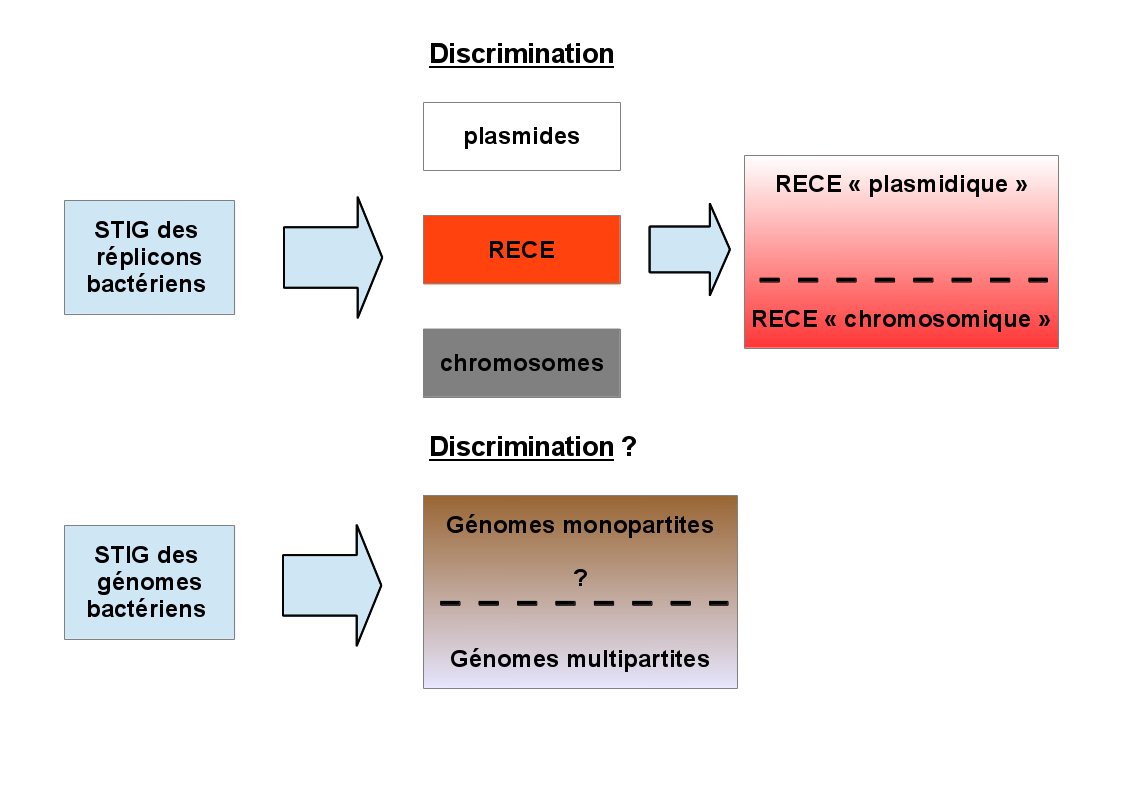
\includegraphics[width=0.9\textwidth ]{./img/schema_discussion.png}
	\caption{Synthèse des résultats.}\label{figresschema}
\end{figure}
      
      Ces biais ont été établis sur la base d'unités structurales, les clusters de protéines homologues, et fonctionnelles, par le choix des protéines selon leurs liens avec les STIG. Bien que la discrimination entre RECE, chromosomes et plasmides soit nette, celle entre génomes mono- et multipartites est plus floue. Parmi les RECE, différents types de biais sont observés: un biais fort caractérisé par la présence de nombreux gènes de type chromosomique, notamment détectable pour les RECE de \textit{Prevotella, Anabaena, Asticcacaulis} et \textit{Paracoccus}, et un biais moins marqué en comparaison des distributions des gènes des STIG des plasmides, observable en particulier pour les RECE de \textit{Deinococcus, Leptospira} et \textit{Cyanothece}. Enfin, les critères fonctionnels (\textit{i.e.}, les annotations) semblent permettre une meilleure discrimination que les critères structuraux (\textit{i.e.}, les clusters de protéines homologues), suggérant que \textbf{les RECE sont mieux définis par les fonctionnalités de leurs STIG que par l'histoire évolutive de leurs gènes}. 
  	
		
\subsection{Implications de la discrimination des RECE par les STIG}	
	La présence sur un RECE d'un gène supplémentaire codant une fonction donnée a plusieurs implications possibles quant au rôle et au devenir de ce gène. Par exemple, un gène sur un RECE peut être soumis à de contraintes évolutivess moins fortes que sur le chromosome et ainsi, acquérir une nouvelle fonction plus facilement au sein de l'organisme (\textit{cf.} Chapitre 2 \S  \ref{chrIIfunc}). Un biais en gènes chromosomiques sur un RECE peut alors d'une part, être la conséquence d'échanges génomiques favorisés par la cohabitation durable entre RECE et chromosome et, d'autre part, refléter un mécanisme évolutif spécifique des génomes multipartites bactériens. Un biais en gènes plasmidiques sur les RECE, par rapport aux chromosomes, peut refléter les origines plasmidiques des RECE. Cependant, l'intégration des RECE dans le génome stable requiert le développement de mécanismes génétiques supplémentaires, dont certains ont déjà été caractérisés (\textit{cf.} Chapitre 2 \S \ref{model}). Ainsi, \textbf{on peut légitimement se demander si les biais observés en gènes des STIG présents sur les RECE sont des conséquences des origines évolutives de ces éléments génomiques et de leur cohabitation avec le génome stable, ou bien reflètent l'adaptation des mécanismes des STIG des génomes multipartites permettant l'intégration des RECE dans le cycle cellulaire}. Ci-dessous sont donnés divers arguments en faveur de cette seconde hypothèse:
\begin{description}
		\item[$\blacktriangleright$] Des biais en gènes essentiels sur un ensemble de RECE ont déjà été caractérisés mais, contrairement aux gènes des STIG, aucune  tendance globale n'a été identifiée \citep{Harrison2010,harrison2011bacterial}.
		 \item[$\blacktriangleright$] Il existe des mécanismes d'adaptation fonctionnelle communs à des génomes multipartites provenant de différentes lignées bactériennes, tels que l'adaptation du système \textit{parABS} chez les Burkholdériales et chez \textit{V. cholerae} (\textit{cf.} Chapitre 2 \S \ref{model}) mais aussi chez certains plasmides des Rhizobiales, qui possédent un système \textit{repABC} singulier. Ces systèmes sont présents de facon très majoritaire sur des mégaplasmides à bas taux de copies ayant un rôle important dans la \textit{fitness} des cellules ainsi que sur certains RECE \citep{Cervantes-Rivera2011,Petersen2013}. Il est alors raisonnable de supposer que ces systèmes contribuent à la stabilisation des réplicons accessoires dans le génome. Nos analyses permettent d'identifier un biais significatif en gènes codant des fonctions annotées \textit{parA/parB} (\textit{cf.} Chapitre 6 \S \ref{reglogresult}). Cette caractéristique est par exemple retrouvée sur les RECE des \textit{Leptospira} ou de \textit{Deinococcus} (\textit{cf.} Chapitre 5 \S \ref{graphres}), laissant supposer que l'adaptation des systèmes \textit{parABS}, ou de manière plus générale des systèmes de partition, est une condition \textit{sine qua non} de la stabilisation des réplicons.
		 \item[$\blacktriangleright$] Certains gènes ayant des annotations telles que celles correspondant aux initiateurs de la réplication chromosomique \textit{dnaA}, ou encore à \textit{ftsZ}, sont présents de façon quasi ubiquiste sur les chromosomes. Au contraire, les gènes codant pour les réplicateurs plasmidiques Rep se trouvent de facon très minoritaire sur les chromosomes. Ces biais suggèrent alors que la présence de gènes des STIG sur un réplicon bactérien sont liés à des mécanismes des STIG spécifiques.   
		 \item[$\blacktriangleright$] Les chromosomes peuvent être classés selon la taxonomie de leur hôte en utilisant des marqueurs génétiques de type ARNr reflétant l'évolution verticale de ces réplicons. Un groupe taxonomique de chromosomes (par exemple une espèce) reflète alors les caractéristiques fonctionnelles et structurales communes de ces génomes. Contrairement aux chromosomes, les plasmides représentent des unités génomiques fonctionnelles et structurales qui sont soumises fortement aux THG et pour lesquelles il est plus difficile de trouver des critères génétiques de classification. Il a été suggéré qu'une partie des gènes des STIG, les recombinases, les systèmes de partition des réplicons et d'initiation de la réplication (\textit{cf.} Chapitre \ref{chap1a} et Chapitre 2 \S \ref{parmodelepl}),  présents sur les plasmides pouvaient servir à classer ces réplicons dans différentes classes taxonomiques et fonctionnelles. Ces propositions  se trouvent confirmées par les résultats des analyses de clustering où différents groupes de plasmides, liés à la taxonomie, sont retrouvés (\textit{c.f.} \S \ref{parmodelepl}). 
\end{description}
	
	
\subsection{Études complémentaires}
\begin{description}
\item[$\blacktriangleright$] Les biais des STIG mis en évidence et caractérisés dans cette étude ont révélé certains phénomènes qu'il est nécessaire de caractériser \textit{via} des analyses complémentaires.
    \begin{description}
     \item[$\bullet$] L'inclusion de davantage de fonctions liées directement ou indirectement aux STIG permettrait d'une part de mieux caractériser les génomes de certaines espèces pour lesquelles les modèles des STIG sont encore incompris et incomplets. D'autre part, certaines fonctions indirectes des STIG, telles que les réplicases ou les systèmes de conjugaison, n'ont pas été prises en considération dans notre étude. Les inclure dans un second temps peut apporter des éléments supplémentaires de comparaison. Enfin, l'inclusion des gènes liés au génome-cœur peut aussi permettre de comparer les biais pour ces gènes avec ceux observés pour les seuls STIG.
     \item[$\bullet$] De même que pour à l'analyse des réplicons par la recherche d'homologues des STIG, il semble pertinent d'inclure dans l'analyse les motifs structurels dont le rôle est lié aux STIG (\textit{cf.} Chapitre 1 \S \ref{motifstruc}). Cependant, l'identification et l'annotation de motifs soulèvent des difficultés techniques, et une expertise spécifique dans la détection de motifs est nécessaire du fait de leur taille réduite ($\simeq 50 pb$ généralement) et de leur variabilité. Dans l'objectif de caractériser les sites \textit{dif} des RECE des \textit{Prevotella}, des analyses ont été menées parallèlement sans succès. En utilisant les sites \textit{dif} déjà caractérisés de génomes d'espèces proches, il nous a été impossible d'identifier avec certitude les positions exactes des sites \textit{dif} sur ces réplicons (résultats non montrés).
     \item[$\bullet$] La structure de la séquence \textit{ori} d'origine de réplication des réplicons bactériens organisée en interne en motifs fonctionnels et, sur le réplicon, à proximité de certains gènes refléte le type du réplicon (\textit{cf.} Chapitre 1 \S \ref{oristruct}). Inclure ces données dans l'analyse permettrait d'obtenir des paramètres supplémentaires liés à la stabilisation des réplicons dans le génome.
    \end{description}	
     
L'ensemble de ces études complémentaires peuvent alors servir à construire un modèle mixte, fondé sur des caractéristiques fonctionnelles et structurales, qui permettrait de mieux caractériser les réplicons bactériens. 
\item[$\blacktriangleright$] Par ailleurs, l'analyse de synténie du Chapitre \ref{chapsynt} révèle certaines spécificités de la structure des RECE. Une analyse globale de synténie sur l'ensemble des réplicons bactériens devrait permettre de les affiner et de les caractériser précisément. 
\item[$\blacktriangleright$] Enfin, les analyses des Chapitres \ref{chap2} et \ref{chap6} montrent qu'il existe un biais des STIG présents entre génomes monopartites et génomes multipartites. Ces différences impliquent notamment des gènes liés à la régulation (de type \textit{iciA} et \textit{lrp}). Des études complémentaires, expérimentales ou analytiques, sont donc nécessaires pour confirmer ou infirmer l'importance de ces fonctionnalités et avancer dans la connaissance des processus cellulaires.
\end{description}	
	


\section{Remise en cause des hypothèses sur la nature des chromosomes secondaires}\label{chromidefaux}
 
    Bien que le concept de \textit{chromid} soit intéressant pour décrire une partie des RECE (chez les Protéobactéries), différentes exceptions et contre-exemples existent. \\
    Le critère d'identification du biais nucléotidique n'est pas universellement vrai. Chez \textit{Cyanothece}, le RECE linéaire a un pourcentage en G+C de 38.6\% comparé aux 37.9\% du chromosome et 38.6\%, 41.5\%, 38.1\% et 37.0\% des plasmides additionnels \citep{Welsh2008}. De même, le RECE de \textit{Thermobaculum terrenum} a un pourcentage en G+C de 64\% par opposition aux 48\% du chromosome \citep{Kiss2010}. Dans un dernier temps, le modèle du \textit{chromid} n'autorise pas d'autre hypothèse évolutive que l'hypothèse \textbf{H2}, qui décrit l'apparition des RECE \textit{via} l'enrichissement de plasmides originels (\textit{cf.} Chapitre 2 \S \ref{chrIIori}).\\ 
    Bien que des cas de formation de RECE relevant de l'hypothèse \textbf{H1}, expliquant la formation de RECE par la scission d'un chromosome originel, n'aient pas été formellement montrés, des données expérimentales de réarrangement génomique indiquent que cette modalité ne peut être rejetée. Le génome de \textit{B. cereus} peut exister en un unique et large chromosome ou sous la forme d'un chromosome plus petit et de réplicons additionnels correspondant à des fragments du chromosome principal \citep{carlson1994small}. Inversement, il a été montré que des réplicons accessoires peuvent intégrer le chromosome chez \textit{S. meliloti} \citep{guo2003natural}.
Les résultats concernant l'analyse par les STIG ainsi que les analyses de synténie des génomes d'\textit{Asticcacaulis}, de \textit{Deinococcus}, de \textit{Prevotella} et d'\textit{Anabaena} contrastent fortement avec les résultats obtenus avec les génomes multipartites ``classiques", les plus étudiés et mieux caractérisés tels que ceux des Vibrionales et des Burkholdériales, et laissent envisager qu'ils sont issus d'un mécanisme de formation, autre que \textbf{H2}, compatible avec \textbf{H1}.\\   
     Enfin, étant donné que les génomes présentant des RECE sont disséminés dans l'ensemble du domaine bactérien, {\color{orange}\textbf{il est probable que les apparitions des génomes multipartites dans les différentes lignées bactériennes sont le fruit d'événements évolutifs distincts}}. Il est alors raisonnable de concevoir qu'au moins un organisme bactérien a acquis un second chromosome selon une autre modalité que celle proposée par l'hypothèse \textbf{H2}.   
\\
La formation d'un RECE peut ne pas impliquer les plasmides comme vecteurs de réplicons additionnels. Le modèle du \textit{chromid} développé par Harisson \textit{et al.} n'est pas applicable dans l'ensemble des cas. La terminologie de ``chromosome secondaire" est ainsi plus adaptée car elle ne préjuge pas d'un mode de formation particulier des RECE. Cependant, elle laisse présupposer qu'il existe un chromosome principal formé antérieurement aux RECE. Dans le cas de la formation de RECE selon les modalités de l'hypothèse \textbf{H1}, cette appellation n'est pas applicable car les deux chromosomes ont été formés de facon simultanée, lors de la scission du chromosome originel. La terminologie de \textbf{néo-chromosomes} apparaît alors mieux adaptée pour décrire les RECE et chromosome ainsi formés car elle place sur un pied d'égalité l'ensemble des réplicons essentiels néo-formés du génome.
    
    
   
\section{Origine des biais de distribution des gènes des STIG}
	Plusieurs mécanismes génétiques peuvent être envisagés pour expliquer la singularité des distributions des gènes des STIG sur les RECE. Le résultats présentés dans le Chapitre \ref{chapsynt} permettent de proposer des éléments de réponse.
\begin{description}
	\item[$\bullet$] \textbf{Transfert latéral intra-génomique.} Ces mécanismes impliquent que les RECE ont acquis des gènes des chromosomes ou des plasmides \textit{via} un échange intra-génomique et que le gène transféré du réplicon ``donneur" est présent \textit{uniquement} sur le RECE. Ces phénomènes ont été décrits pour les génomes multipartites des \textit{Burkholderia} et des Rhizobiales notamment (\textit{cf.} Chapitre 8 \S \ref{parbruc} et \S \ref{parburk}).
	\item[$\bullet$] \textbf{Duplication suivie de transfert intra-génomique.} Ce mécanisme est similaire au précédent mais une copie du gène des STIG présent sur le RECE est aussi présent sur le réplicon ``donneur", de façon analogue au mécanisme de paralogie. La présence d'une copie supplémentaire de gène annoté \textit{hfq} sur les RECE des \textit{Burkholderia} a été rapportée (\textit{cf.} Chapitre 6 \S \ref{reglogresult}).
	\item[$\bullet$] \textbf{Coupure du réplicon.} Ce mécanisme implique la coupure d'un réplicon originel donnant naissance à deux réplicons fonctionnels. L'acquisition de STIG fonctionnels pour chacun des deux nouveaux réplicons passe par l'intégration de modules génétiques externes, par exemple plasmidiques. Il n'existe pas actuellement de recensement et de description précise de ce type de formation de réplicon chez les bactéries. Néanmoins, un tel mécanisme a été suggéré par divers auteurs (\textit{cf.} Chapitre 2 \S \ref{chrIIori}), et \textit{in vitro} chez \textit{B. cereus}, le chromosome a été expérimentalement scindé en deux réplicons stables \citep{itaya1997experimental}. Le fort biais en gènes des STIG observés sur certains RECE ainsi que les résultats des analyses de synténie (Chapitre \ref{chapsynt}) font supposer que les RECE de \textit{Prevotella, Paracoccus, Asticcacaulis} et \textit{Anabaena} ont été formés selon cette modalité.
	\item[$\bullet$] \textbf{Transfert latéral inter-génomique.} L'acquisition de gènes des STIG étrangers au génome \textit{via} des THG est un mécanisme à l'origine des biais observés sur les RECE. Une partie des gènes présents sur un réplicon extra-chromosomique  d'\textit{Azospirillum brasilense} CBG497 caractérisés comme potentiels RECE,  sont des orthologues de gènes de génomes d'espèces, genres ou phyla différents (xénologues), dont deux codent une transposase \citep{Acosta-Cruz2012}.
	\item[$\bullet$] \textbf{Fusion de deux réplicons.} Dans certains cas, un réplicon peut s'intégrer au sein d'un autre. Ces observations ont été faites \textit{in vitro}, chez \textit{E. coli} \citep{bernander1991coli} par exemple et \textit{in vivo} où il a notamment été reporté que certains RECE pouvaient intégrer de facon stable le chromosome (\citep{guo2003natural}). Récemment, il a été montré \textit{in vitro} que la réplication du RECE de \textit{Vibrio cholerae} sans l'intervention de Dam et RtcB est possible par la fusion du RECE avec le chromosome, la réplication s'effectuant \textit{via} la machinerie moléculaire du chromosome \citep{val2014fuse}.
\end{description}  
	
	
	
\section{Proposition d'un modèle moléculaire d'origine des néo-chromosomes} 
	On peut alors supposer que ces différents mécanismes génétiques sont grandement impliqués dans la diversification des STIG chez les réplicons bactériens. Ils peuvent par exemple contribuer à la \textit{replicon takeover hypothesis}, selon laquelle un réplicon accessoire peut rendre fonctionnelle sa machinerie réplicative par intégration au sein d'un autre réplicon, chromosome ou plasmide \citep{mcgeoch2008extra}. Par exemple, l'intégration \textit{in vitro} d'un plasmide R1 au sein du chromosome d'\textit{E. coli} a pu rendre inutile l'action de DnaA, la réplication se faisant \textit{via} l'origine et les initiateurs du plasmide intégré \citep{bernander1991coli}. On peut aussi rapprocher de cette hypothèse le cas des réplicons contenant de multiples origines de réplication actives (ou plus exactement, des éléments génomiques à multiple réplicons), comme par exemple chez certains plasmides (\textit{cf.} \S \ref{architecture}) qui bénéficient ainsi d'un large spectre d'hôtes \citep{Toukdarian2004}. \\
	Des mécanismes de régulation sont à l'oeuvre entre le chromosome et le mégaplasmide chez \textit{Streptomyces clavuligerus} (Actinobactéries) et font vraisemblablement intervenir des protéines plasmidiques héritées du chromosome \textit{via} des mécanismes de recombinaison ou de transposition \citep{medema2010sequence}. Le taux élevé de gènes de type \textit{recA}, codant pour une protéine impliquée dans la réparation de l'ADN, dans le génome d'\textit{Acaryochloris marina} (Cyanobactéries) a probablement contribué à l'expansion de son génome, ces gènes étant apparus par duplication et/ou THG \citep{swingley2008niche}. Enfin, un dernier exemple intéressant est l'hypothèse selon laquelle certains systèmes de conjugaison seraient d'abord apparus chez les Protéobactéries puis auraient été diffusés horizontalement dans l'ensemble des lignées bactériennes ainsi que chez les Archées \citep{Guglielmini2013}. En particulier, TraB, protéine appartenant aux systèmes de sécrétion de type IV, et FtsK, protéine majeure du fonctionnement cellulaire liant la réplication des réplicons à la division cellulaire, dériveraient d'une protéine ancestrale commune \citep{Vogelmann2011}.\\
	 \textbf{\color{orange} La distribution des gènes des STIG sur les réplicons bactériens forment ainsi un marqueur pertinent de la stabilisation et de l'intégration des réplicons dans le génome bactérien et témoigne des spécificités des réplicons.} Le passage d'une architecture génomique monopartite à une architecture multipartite requiert des STIG spécifiques, que notre étude des caractéristiques discriminantes des RECE a mis en évidence. En considérant l'ensemble des génomes, il semble de plus que le bon fonctionnement des génomes multipartites par rapport aux génomes monopartites réclame le soutien de gènes supplémentaires, impliqués dans la régulation (régulateurs de type \textit{iciA} ou \textit{lrp}) ou intervenant dans la partition.
	 
     %évolution réticulaire: conjugaison: évolution à partir d'un groupe de gènes et se retrouve sur plasmides et transposons \citep{thomas2005mechanisms}. Voir aussi \citep{mochizuki2006genetic}
     %Évolution des génomes associés aux plantes, trouver un peu de biblio.
     
\section{Continuité du matériel génomique}\label{continuite}
     L'exemple de la propagation de systèmes de conjugaison à travers l'ensemble des lignées bactériennes à partir d'un système originel limité initialement à un seul groupe d'espèce illustre bien la notion de continuité du matériel génomique. Certains indices génomiques montrent que des protéines similaires liées aux STIG, vraisemblablement héritées de protéines ancestrales communes, existent chez les Archées, Eucaryotes et Bactéries \citep{mcgeoch2008extra}. \textbf{\color{orange} Parallèlement à l'évolution des systèmes génétiques, l'étude des réplicons bactériens permet de mettre en avant la continuité du matériel génomique.} Chez les réplicons de \textit{B. subtilis} ainsi que dans d'autres génomes bactériens, des mégaplasmides ont été formés à partir de la fusion de petits plasmides, ce mécanisme pouvant être une cause majeure de formation de mégaplasmide chez les bactéries \citep{zheng2013evolution}. Il existe alors non seulement une plasticité génétique des réplicons mais aussi de leur degré de stabilisation dans le génome. Tout comme plasmides et chromosomes, les RECE et néo-chromosomes sont des espèces génomiques marqueurs de processus spécifiques d'intégration et de complexification (ou \textit{dés}intégration et réduction) des génomes bactériens.  
     
     
  
     
 %\section{Implication pour la définition d'une espèce bactérienne}
 % \emph{Peut-être enlever ce paragraphe car finalement pas grand chose à dire de pertinent}\\
 %   Sachant qu'un individu bactérien est défini par son génome, composé de réplicons stables et instables, soumis à des échanges intra et inter génomiques avec d'autres individus plus ou moins proches génétiquement, comment peut-on définir une espèce bactérienne? Définition de la littérature \cite{Lawrence2009,Doolittle2007}, réflexions personnels dessus.
    
    
  
